\subsection{Oceanía}

Comenzamos la experimentación analizando la ruta a la Universidad de Sydney (www.sydney.edu.au). Se adjunta lo devuelto por la herramienta. Nuestra hipótesis para este caso es que exiten dos saltos intercontinentales. \\

\begin{tabular}{ |p{1cm}||p{3cm}|p{2cm}|p{2cm}|p{2cm}|p{1.5cm}|  }
 \hline
 \multicolumn{5}{|c|}{Traceroute a Sydney} \\
 \hline
 \textit{TTL} & \textit{IP}  & \textit{RTT} & $\delta$\textit{RTT}&\textit{ZRTT} & Outlier? \\
 \hline
1 &  192.168.1.1  &  2.3 ms  & - & - \\    
2 &  201.212.34.1   & 31.47 ms &  29.16 ms    &     0.29    & \\  
3  &  Sin Respuesta  &  -   &   -    &   -  & \\   
4   & Sin Respuesta  &  -   &   -   &    -  & \\ 
5    & Sin Respuesta  & -    &   -   &    -    & \\ 
6  &  200.89.161.97  & 24.76 ms &  -    &   -    & \\ 
7   & 200.89.165.197 & 31.78 ms &  0.31 ms    &      0.96     & \\ 
8   & 200.89.165.222 & 28.39 ms &  -    &      -        & \\ 
9   & Sin Respuesta  &  -    &   -   &      -       & \\ 
10  & 67.17.94.249   & 147.04 ms & 115.26 ms   &     1.69     &         OUTLIER! \\
11  & Sin Respuesta  &  -   &   -   &      -       & \\  
12  & Sin Respuesta  &  -  &   -    &       -      & \\ 
13  & 4.68.127.54    & 145.73 ms &  -           &     -        & \\ 
14  & 129.250.2.202  & 179.17 ms &    32.13 ms   &      0.23    & \\ 
15  & 129.250.4.250  & 150.88 ms &   -           &     -        & \\ 
16  & 129.250.2.219  & 172.07 ms &   -           &     -        & \\ 
17  & 129.250.7.69   & 188.14 ms &   8.97 ms    &      0.76     & \\ 
18  & 129.250.3.123  & 187.04 ms &   -          &      -        & \\ 
19  & 204.1.253.166  & 227.14 ms &   38.99 ms    &     0.07      & \\ 
20  & 202.158.194.172 & 351.84 ms &    124.71 ms   &     1.9       &        OUTLIER! \\
21  & 113.197.15.68   & 358.21 ms  &    6.36 ms     &     0.82      & \\
22 &   113.197.15.66  & 343.53 ms &     -          &      -        & \\ 
23  & 113.197.15.152  & 379.73 ms &    21.52 ms    &     0.47      & \\ 
24  & 138.44.5.47     & 360.62 ms &    -          &      -         & \\ 
25 &  Sin Respuesta   &  -   &      -        &       -        & \\ 
26 &  Sin Respuesta   &  -  &       -        &      -        & \\ 
27 &  129.78.5.11  &     360.65 ms  &    -         &       -          & \\
 \hline
\end{tabular}

\smallskip

La primer IP corresponde a una dirección privada. Esta es la del router del hogar de uno de los integrantes. La siguiente pertence a la ISP del integrante. Luego no responden 3 hops y tras ello, se observa un cluster con 200.89 como prefijo todos dentro de la Argentina y con RTTT similares.
EL proximo hop, 67.17.94.249 demora mucho más que el resto y la herramienta de geolocalización lo ubica e algún lugar indefinido dentro de Estados Unidos (aunque reporta como hostname una cadena alfanumerica con MIA como subcadena con lo que intuimos que se puede tratar de Miami). 4.68.127.54 también tiene como subcadena de hostanem a miami. LUego se agrupa un cluster 129.250 de tiempo de respuesta similar y se corresponden con la region de Texas y Colorado con lo cual los paquetes se mueven al oeste.\\

\begin{figure}[H]
\centering
\caption{Sydney RTT cada salto}
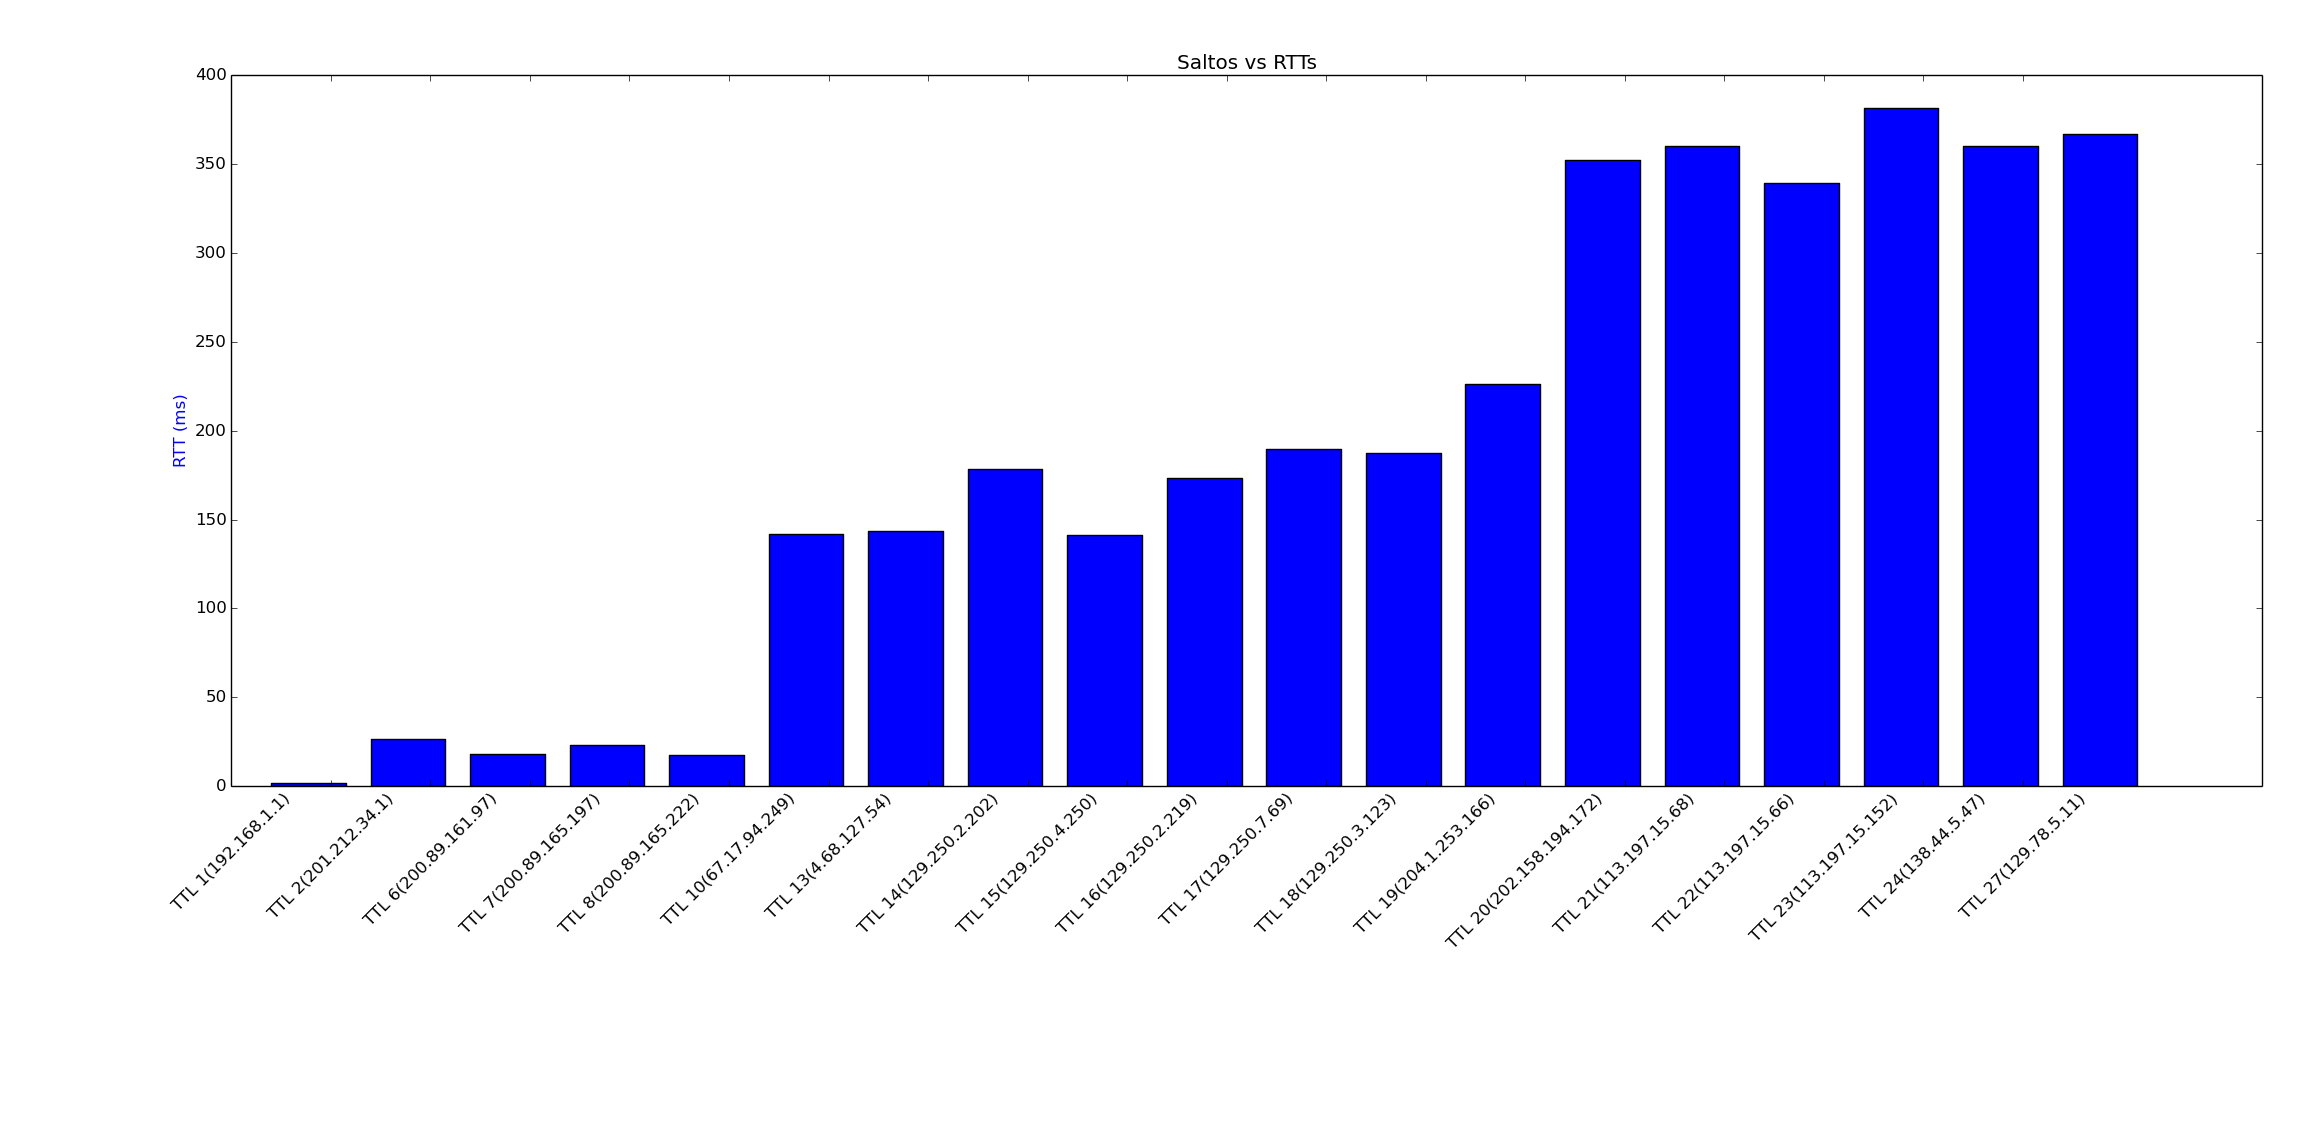
\includegraphics[width=0.7\textwidth]{modules/asia_rtt}
 \label{fig:dysney_rtts}
\end{figure}

Con el salto 202.158.194.172 llega a Perth, al oeste de Australia. 
 El cluste de las ips 113.197 corresponde a Canbeerra y finalmente 129.78.5.11 a la Universidad de Sydney.\\


\begin{figure}[H]
\centering
\caption{Saltos más relevantes según el geolocalizador}
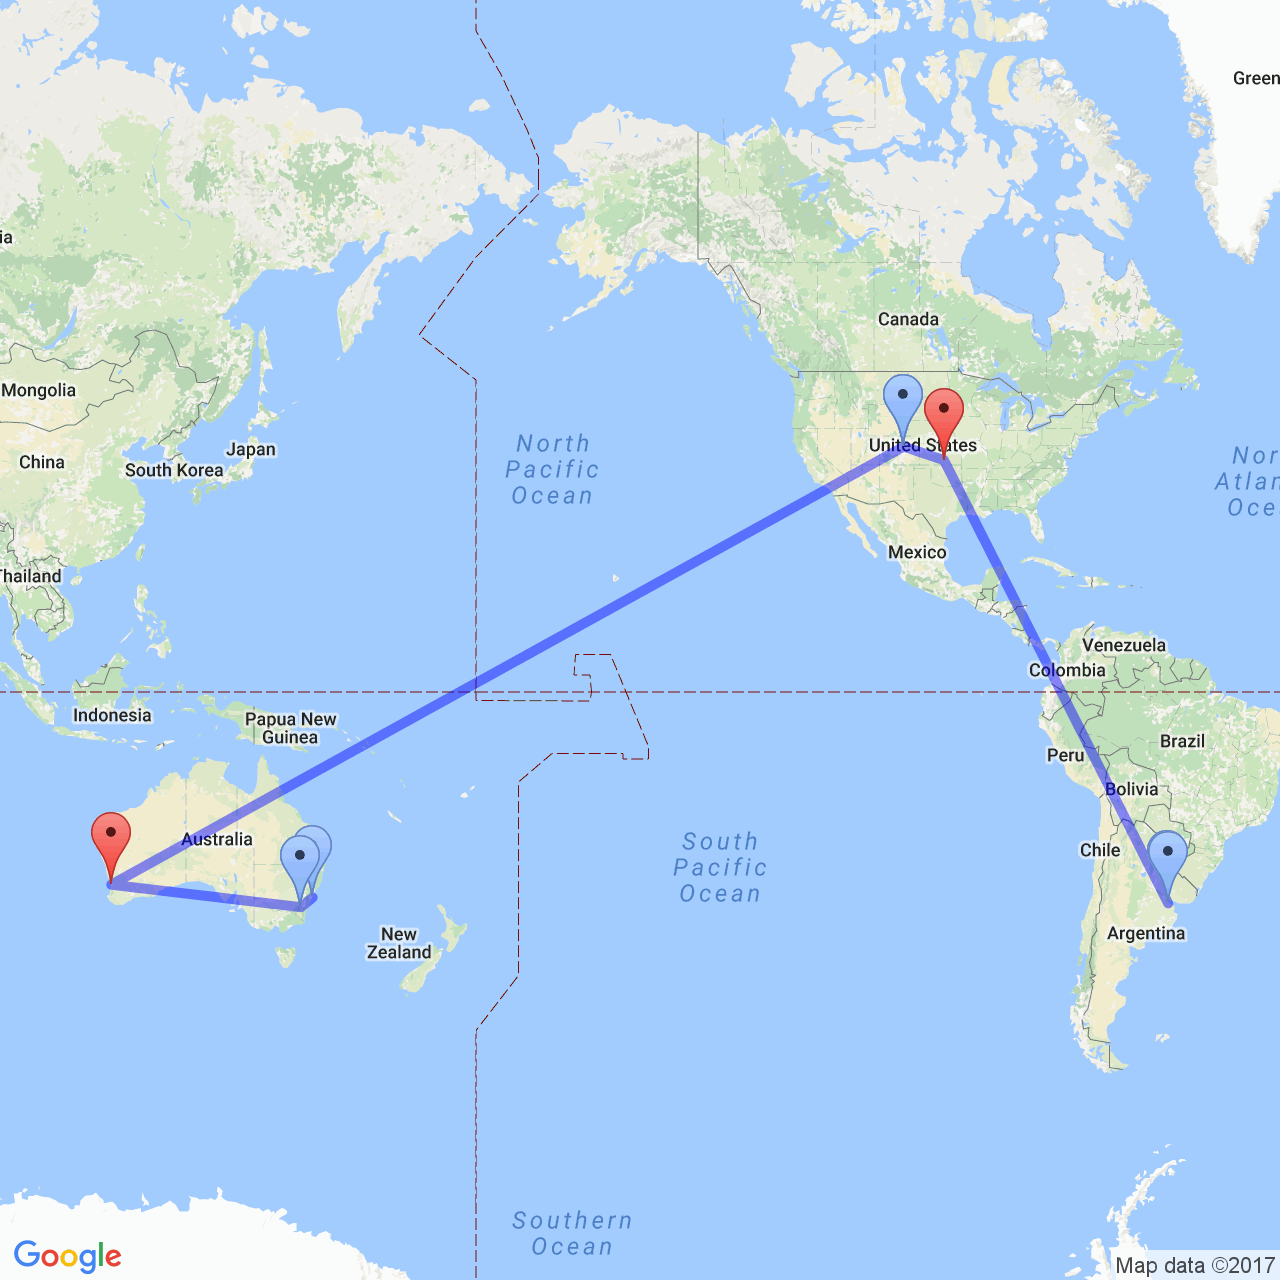
\includegraphics[width=0.7\textwidth]{modules/asia_mapa}
 \label{fig:dysney_mapa}
\end{figure}

Nuestra conjetura es que los saltos 10 y 20 son intercontinentales visto la diferencia de RTTT respecto a los otros.Se observa que el método de Cimbala los detecta como outliers.

\begin{figure}[H]
\centering
\caption{Sydney Delta RTT}
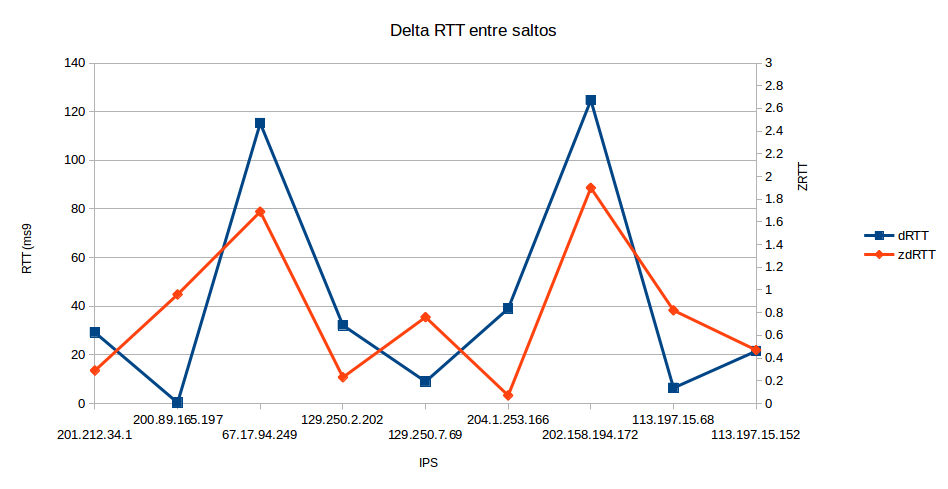
\includegraphics[width=0.7\textwidth]{modules/asia_delta}
 \label{fig:dysney_rtts}
\end{figure}

De esta manera, el métood de Cimbala descarta a dichos saltos cuyos 
ZRTT son mayores a la función $\tau$ de Thompson en n= 9 y 8 
respecivamente (que son la cantidad de saltos tenidos en cuenta, es 
decir los $\Delta RTT$ cuyo valor es positivo respecto al máximo 
anterior en el camino hacia ese salto, tal como hemos comentado en la 
sección anterior.
En el gráfico también se aprecian los ZRTT que esperablemente aumentan a mayor delta, y que son los los hops descartados por Cimbala.\\
Concluimos entonces que para esta experiencia, se corroboró empíricamente que los saltos 10 y 20 eran intercontinentales con dirección IP 67.17.94.249 y 202.158.194.172 respectivamente.
 






